% 请确保文件编码为utf-8,使用XeLaTex进行编译,或者通过overleaf进行编译

\documentclass[answers]{exam}  % 使用此行带有作答模块
% \documentclass{exam} % 使用此行只显示题目

\usepackage{xeCJK}
\usepackage{zhnumber}
\usepackage{graphicx}
\usepackage{hyperref}
\usepackage{amsmath}
\usepackage{booktabs}
\usepackage{enumerate}

\pagestyle{headandfoot}
\firstpageheadrule
\firstpageheader{南京大学}{数字信号处理}{习题集一}
\runningheader{南京大学}
{数字信号处理}
{习题集一}
\runningheadrule
\firstpagefooter{}{第\thepage\ 页(共\numpages 页)}{}
\runningfooter{}{第\thepage\ 页(共\numpages 页)}{}

% no box for solutions
% \unframedsolutions

\setlength\linefillheight{.5in}

% \renewcommand{\solutiontitle}{\noindent\textbf{答:}}
\renewcommand{\solutiontitle}{\noindent\textbf{解:}\par\noindent}

\renewcommand{\thequestion}{\zhnum{question}}
\renewcommand{\questionlabel}{\thequestion .}
\renewcommand{\thepartno}{\arabic{partno}}
\renewcommand{\partlabel}{\thepartno .}


\begin{document}
\Large

\begin{questions}
	
\question 本题所提的关系式在很多场合都会遇到:

\begin{parts}
	\part 证明下面的表示式成立:
	\begin{equation} \nonumber
		\sum_{n=0}^{N-1} \alpha^n = 
		\begin{cases}
			N, & \alpha=1 \\
			\frac{1-\alpha^N}{1-\alpha}, & \text{任意复数} \alpha \neq 1
		\end{cases}
	\end{equation}
	该式子常称为有限项和公式。

	\part 证明:若$|\alpha| < 1$,则:
	\begin{equation} \nonumber
		\sum_{n=0}^{\infty} \alpha^n = \frac{1}{1-\alpha}
	\end{equation}
	该式子常称为无限项和公式。

	\part 证明:若$|\alpha| < 1$,则:
	\begin{equation} \nonumber
		\sum_{n=0}^{\infty} n\alpha^n = \frac{\alpha}{(1-\alpha)^2}
	\end{equation}

	\part 假设$|\alpha| < 1$,求:
	\begin{equation} \nonumber
		\sum_{n=k}^{\infty} \alpha^n
	\end{equation}
\end{parts}

\begin{solution}
	\begin{parts}
		\part 当$\alpha=1$时,$\sum_{n=0}^{N-1}\alpha^n=\sum_{n=0}^{N-1}1=N$。\\
		      当$\alpha\neq1$时,令
		      $$S_N=\sum_{n=0}^{N-1}\alpha^n$$
		      则$\alpha S_N=\sum_{n=1}^{N}\alpha^n$
		      于是$$S_N-\alpha S_N=1-\alpha^N $$又因为$\alpha\neq1$,所以
		      $$S_N=\sum_{n=0}^{N-1}\alpha^n=\frac{1-\alpha^N}{1-\alpha} $$
		\part 当$|\alpha|<1$时,有$\sum_{n=0}^{N-1}\alpha^n=\frac{1-\alpha^N}{1-\alpha}$,
		      从而$$\sum_{n=0}^{\infty}\alpha^n=\lim_{N\to\infty}\sum_{n=0}^{N-1}\alpha^n=
		      \lim_{N\to\infty}\frac{1-\alpha^N}{1-\alpha}=\frac{1}{1-\alpha}$$ 
		\part 对$$\sum_{n=0}^{\infty} \alpha^n = \frac{1}{1-\alpha}$$两边求导,得到
		        $$\sum_{n=0}^{\infty} n\alpha^{n-1} = \frac{1}{(1-\alpha)^2}$$两边同时乘以$\alpha$,得到
		        $$\sum_{n=0}^{\infty} n\alpha^n = \frac{\alpha}{(1-\alpha)^2}$$
		\part 注意到$$\sum_{n=k}^{\infty} \alpha^n = \sum_{n=0}^{\infty} \alpha^n - 
		        \sum_{n=0}^{k-1} \alpha^n$$
		      而$\sum_{n=0}^{k-1} \alpha^n=\frac{1-\alpha^k}{1-\alpha}$,从而
		      $$\sum_{n=k}^{\infty} \alpha^n=\frac{1}{1-\alpha}-\frac{1-\alpha^k}{1-\alpha}=\frac{\alpha^k}{1-\alpha}$$
	\end{parts}
\end{solution}

\question 给出下列各时间函数的波形图,注意它们的区别:
\begin{enumerate}[(1)]
	\item $f_1(t) = \sin(\omega t) \cdot u(t)$
	\item $f_2(t) = \sin\left[ \omega (t-t_0) \right] \cdot u(t)$
	\item $f_3(t) = \sin\left[ \omega (t) \right] \cdot u(t-t_0)$
	\item $f_4(t) = \sin\left[ \omega (t-t_0) \right] \cdot u(t-t_0)$
\end{enumerate}

\begin{solution}
	\begin{enumerate}[(1)]
		\item 如图~\ref{fig:q2-1}
		\item 如图~\ref{fig:q2-2}
		\item 如图~\ref{fig:q2-3}
		\item 如图~\ref{fig:q2-4}
	\end{enumerate}
\end{solution}

\begin{figure}
	\centering
	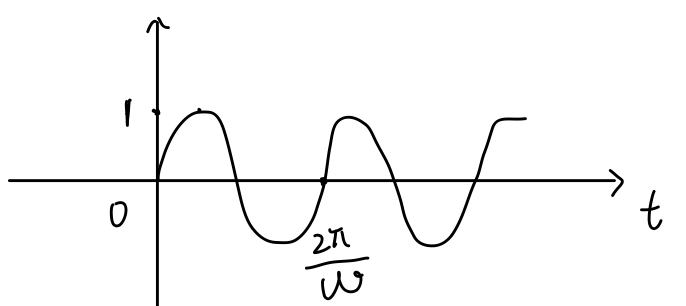
\includegraphics[width=0.5\textwidth]{pics/q2-1.png}
	\caption{$f_1(t)$波形图} \label{fig:q2-1}
\end{figure}
\begin{figure}
	\centering
	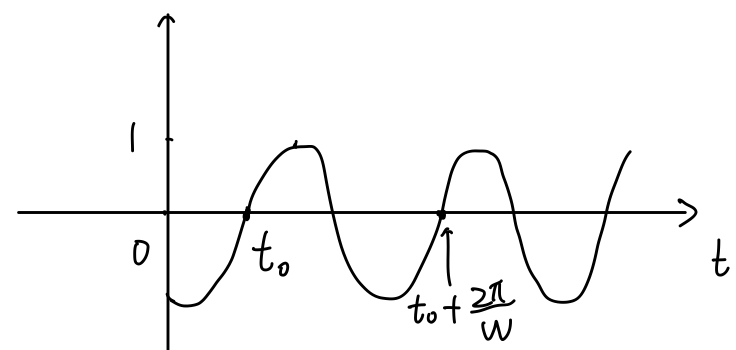
\includegraphics[width=0.5\textwidth]{pics/q2-2.png}
	\caption{$f_2(t)$波形图} \label{fig:q2-2}
\end{figure}
\begin{figure}
	\centering
	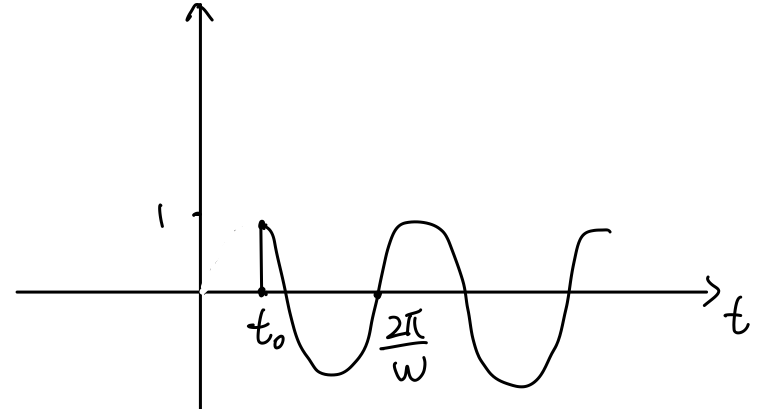
\includegraphics[width=0.5\textwidth]{pics/q2-3.png}
	\caption{$f_3(t)$波形图} \label{fig:q2-3}
\end{figure}
\begin{figure}
	\centering
	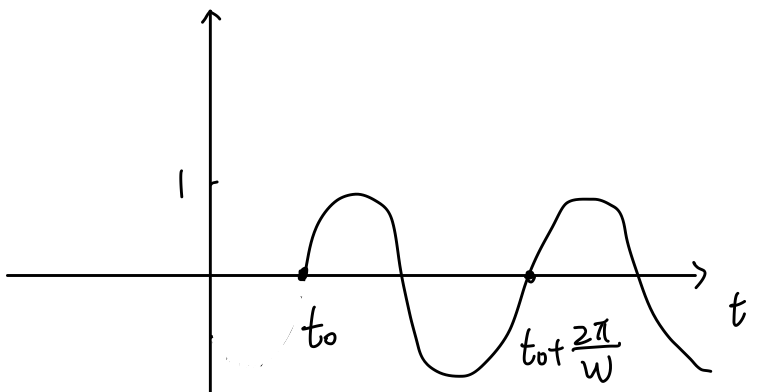
\includegraphics[width=0.5\textwidth]{pics/q2-4.png}
	\caption{$f_4(t)$波形图} \label{fig:q2-4}
\end{figure}

\question 已知$f(5-2t)$的波形如图~\ref{fig:q3-1}所示,画出$f(t)$的波形图。
\begin{figure}
	\centering
	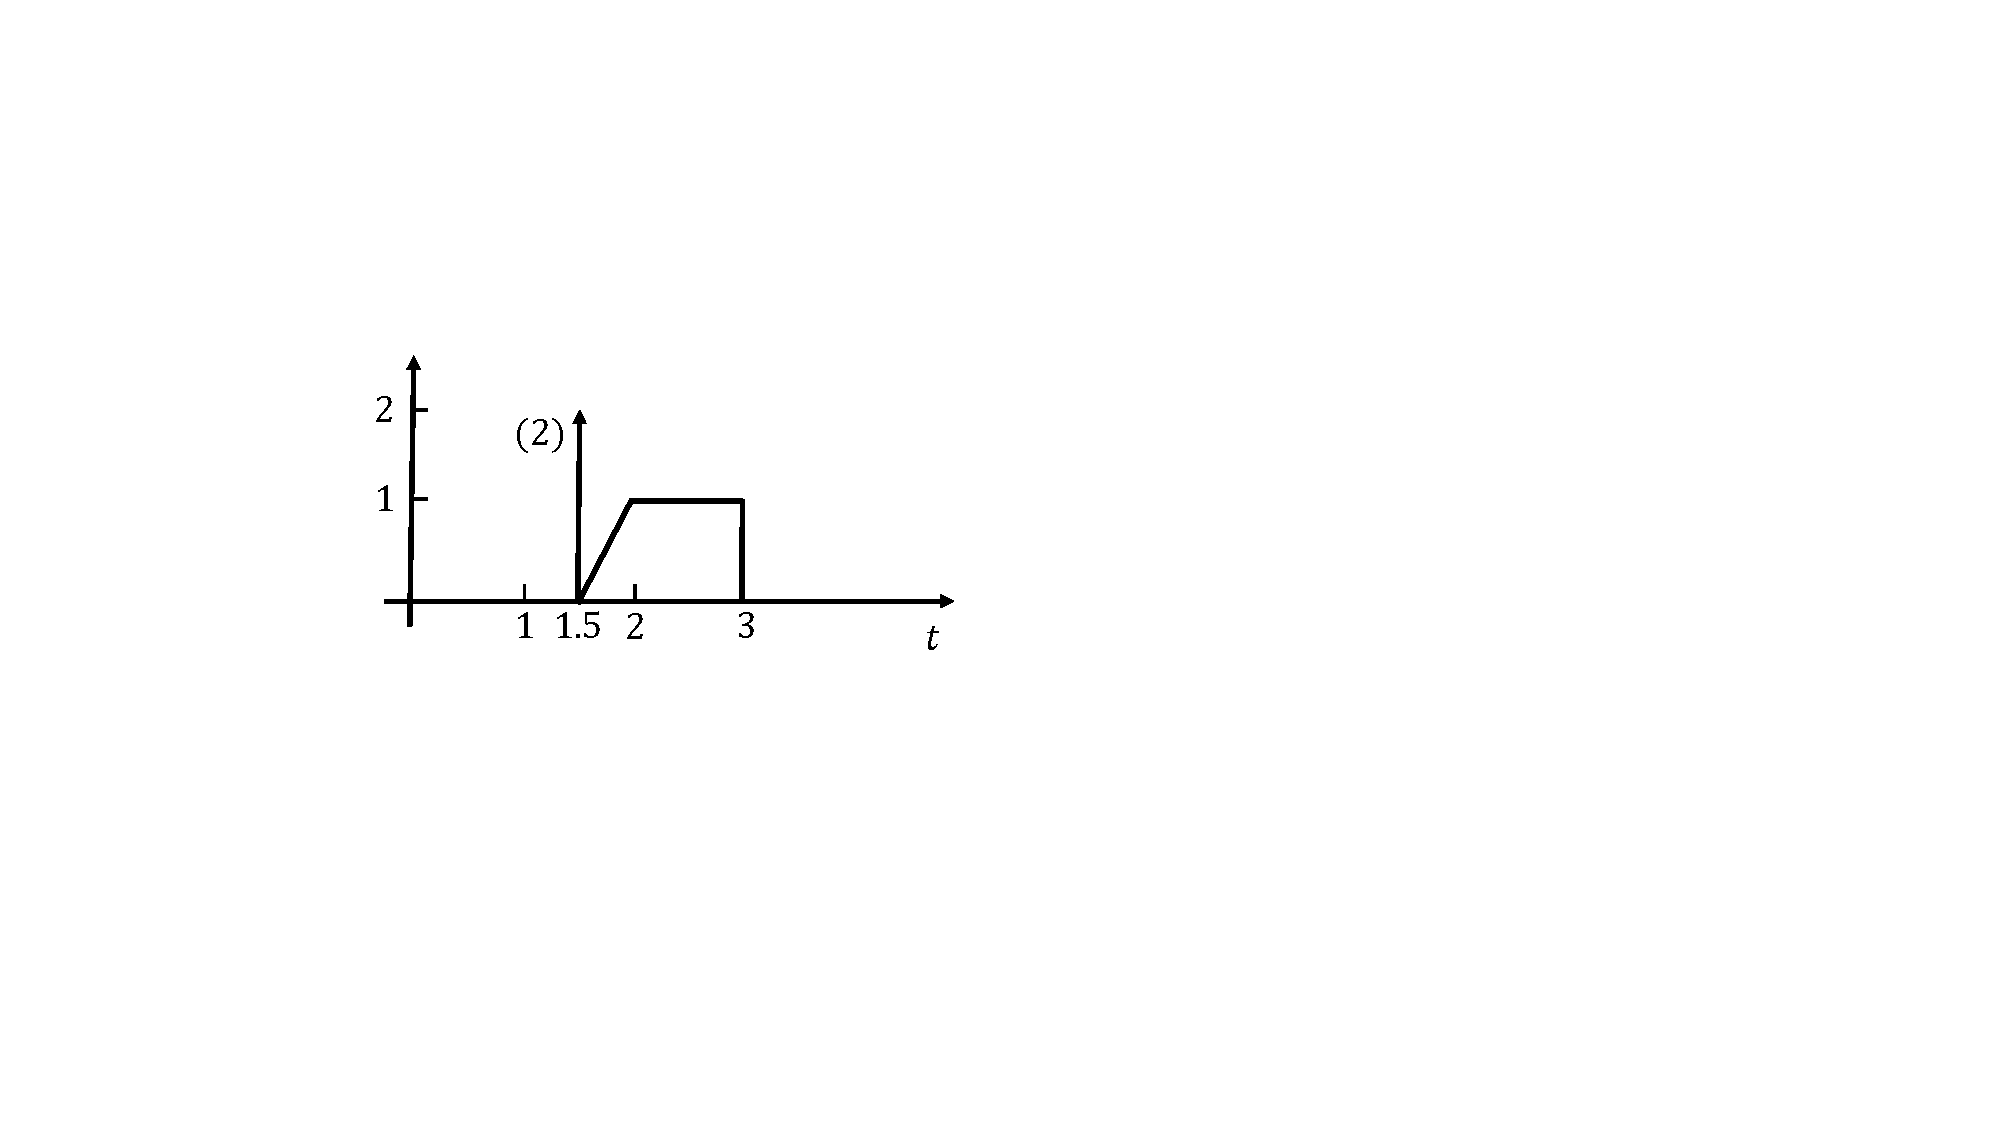
\includegraphics{pics/q2-que.pdf}
	\caption{$f(5-2t)$波形图} \label{fig:q3-1}
\end{figure}

\begin{solution}
	$f(5-2t)=f(-2(t-\frac{5}{2}))$,将原图像左移$\frac{5}{2}$得到$f(-2t)$的图像,再翻转得到$f(2t)$的图像,再扩展到原来的2倍得到$f(t)$的图像如图~\ref{fig:q3-2}:
\end{solution}
\begin{figure}
	\centering
	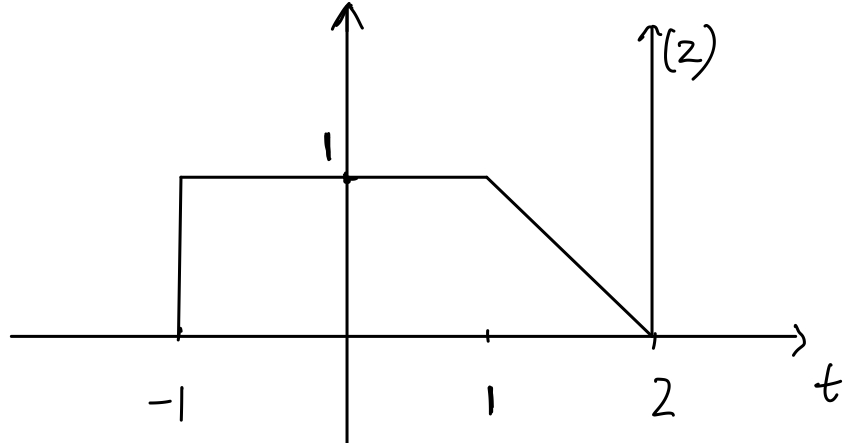
\includegraphics[width=0.5\textwidth]{pics/q3.png}
	\caption{$f(t)$波形图} \label{fig:q3-2}
\end{figure}

\question 分别求下列周期信号的周期$T$:
\begin{enumerate}[(1)]
	\item $\cos(10t)-\cos(30t)$
	\item $e^{j10t}$
	\item $\left[5 \sin(8t) \right]^2$
	\item $\sum_{n=0}^{\infty} (-1)^n \left[ u(t-nT) - u(t-nT-T) \right]$($n$为正整数)
\end{enumerate}

\begin{solution}
	\begin{enumerate}[(1)]
		\item $\cos(10t)$的周期是$T_1=\frac{\pi}{5}$,$\cos(30t)$的周期是$T_2=\frac{\pi}{15}$,$\frac{T_1}{T_2}=3$,所以原周期信号的周期$T=\frac{\pi}{5}$。
		\item $e^{j10t}=\cos(10t)+j\sin(10t)$,$cos(10t)$和$jsin(10t)$的周期均为$\frac{\pi}{5}$,所以原周期信号的周期$T=\frac{\pi}{5}$。
		\item $\left[5 \sin(8t) \right]^2=\frac{25}{2}-\frac{25\cos(16t)}{2}$,所以原周期信号的周期$T=\frac{\pi}{8}$。
		\item 令$f_n(t)=u(t-nT)-u(t-nT-T)$,则
		        \begin{equation} \nonumber
		        	f_n(t) = 
		        	\begin{cases}
		        		1, & nT\leq t<(n+1)T \\
		        		0, & \text{otherwise}
		        	\end{cases}
		        \end{equation}
	          从而$\sum_{n=0}^{\infty}f_n(t)=u(t)$,且容易得到
	          \begin{equation} \nonumber
	          	\sum_{n=0}^{\infty}(-1)^nf_n(t) = 
	          	\begin{cases}
	          		1, & kT\leq t<(k+1)T,k=0,2,4,\cdots \\
	          		-1, & kT\leq t<(k+1)T, k=1,3,5,\cdots\\
	          		0, & t<0
	          	\end{cases}
	          \end{equation}
              当$t\in\mathbf{R}$时,该信号非周期信号;当$t\in[0,\infty)$时,该信号的周期为$2T$。
	          
	\end{enumerate}
\end{solution}


\question 应用冲激信号的抽样特性,求下列表示式的函数值:
\begin{enumerate}[(1)]
	\item $\int_{-\infty}^{\infty} f(t-t_0)\delta(t) dt$
	\item $\int_{-\infty}^{\infty} f(t_0-t)\delta(t) dt$
	\item $\int_{-\infty}^{\infty} \delta(t-t_0)u(t-\frac{t_0}{2}) dt$
	\item $\int_{-\infty}^{\infty} \delta(t-t_0)u(t-2t_0) dt$
	\item $\int_{-\infty}^{\infty} (e^{-t}+t)\delta(t+2) dt$
	\item $\int_{-\infty}^{\infty} (t+\sin t)\delta(t-\frac{\pi}{6}) dt$
	\item $\int_{-\infty}^{\infty} e^{-j\omega t}\left[ \delta(t)-\delta(t-t_0)\right] dt$
\end{enumerate}

\begin{solution}
	以下不妨假设$t_0>0$。
	\begin{enumerate}[(1)]
		\item 原式$=\int_{-\infty}^{\infty} f(0-t_0)\delta(t) dt=
		       f(-t_0)\int_{-\infty}^{\infty} \delta(t) dt=f(-t_0)$
		\item 原式$=\int_{-\infty}^{\infty} f(t_0-0)\delta(t) dt=
		      f(t_0)\int_{-\infty}^{\infty} \delta(t) dt=f(t_0)$
		\item 原式$=\int_{-\infty}^{\infty} \delta(t-t_0)u(t_0-\frac{t_0}{2}) dt=u(\frac{t_0}{2})=1$
		\item 原式$=\int_{-\infty}^{\infty} \delta(t-t_0)u(t_0-2t_0) dt=u(-t_0)=0$
		\item 原式$=\int_{-\infty}^{\infty} (e^{2}-2)\delta(t+2) dt=
		      (e^{2}-2)\int_{-\infty}^{\infty} \delta(t+2) dt=e^{2}-2$
		\item 原式$=\int_{-\infty}^{\infty} (\frac{\pi}{6}+\sin
		\frac{\pi}{6})\delta(t-\frac{\pi}{6})       dt=(\frac{\pi}{6}+\frac{1}{2})\int_{-\infty}^{\infty}\delta(t-\frac{\pi}{6})  dt=\frac{\pi}{6}+\frac{1}{2}$
		\item 原式$=\int_{-\infty}^{\infty} e^{-j\omega t} \delta(t) dt -
		\int_{-\infty}^{\infty} e^{-j\omega t}\delta(t-t_0)dt=1-e^{-jwt_0}$
	\end{enumerate}
\end{solution}


\question 判断下列系统是否是线性的、时不变的、因果的:
\begin{enumerate}[(1)]
	\item $y(t) = \frac{d x(t)}{dt}$
	\item $y(t) = x(t)u(t)$
	\item $y(t) = \sin \left[x(t)\right]u(t)$
	\item $y(t) = x(1-t)$
	\item $y(t) = x(2t)$
	\item $y(t) = x^2(t)$
	\item $y(t) = \int_{-\infty}^t x(\tau) d\tau$
	\item $y(t) = \int_{-\infty}^{5t} x(\tau) d\tau$
\end{enumerate}

\begin{solution}
	\begin{enumerate}[(1)]
		\item 线性系统,时不变系统,因果系统。
		\item 线性系统,时变系统,因果系统。
		\item 非线性系统,时变系统,因果系统。
		\item 线性系统,时变系统,非因果系统。
		\item 线性系统,时变系统,非因果系统。
		\item 非线性系统,时不变系统,因果系统。
		\item 线性系统,时不变系统,因果系统。
		\item 线性系统,时变系统,非因果系统。
	\end{enumerate}
\end{solution}


\question 求下列各个函数$f_1(t)$与$f_2(t)$的卷积$f_1(t)\ast f_2(t)$:
\begin{enumerate}[(1)]
	\item $f_1(t)=u(t),f_2(t)=e^{-at}u(t)$
	\item $f_1(t)=\delta(t),f_2(t)=\cos (\omega t + 45^{\circ})$
	\item $f_1(t)=(1+t)\left[u(t)-u(t-1)\right],f_2(t)=u(t-1)-u(t-2)$
	\item $f_1(t)=\cos(\omega t),f_2(t)=\delta(t+1)-\delta(t-1)$
	\item $f_1(t)=e^{-at}u(t),f_2(t)=(\sin t)u(t)$
\end{enumerate}


\begin{solution}
	\begin{enumerate}[(1)]
		\item $f_1(t)\ast f_2(t)=\int_{-\infty}^{\infty} e^{-a\tau}u(\tau)u(t-\tau) d\tau$。当$t<0$时,卷积为0;当$t\geq0$时,$f_1(t)\ast f_2(t)=\int_{0}^{t} e^{-a\tau}u(\tau)u(t-\tau) d\tau=\frac{1}{a}(1-e^{-at})$。从而$f_1(t)\ast f_2(t)=\frac{1}{a}(1-e^{-at})u(t)$。
		\item $f_1(t)\ast f_2(t)=\int_{-\infty}^{\infty} \delta(t-\tau)\cos (\omega \tau + 45^{\circ})d\tau=\int_{-\infty}^{\infty} \delta(t-\tau)\cos (\omega t + 45^{\circ})d\tau
		=\cos (\omega t + 45^{\circ})$
		\item $f_1(t)\ast f_2(t)=\int_{-\infty}^{\infty} (1+\tau)[u(\tau)-u(\tau-1)][u(t-\tau-1)-u(t-\tau-2)]d\tau$。容易看出,当$0<\tau<1$且$t-2<\tau<t-1$时积分不为0。从而,
		\begin{enumerate}[$\bullet$]
			\item 当$t<1$或$t>3$时,卷积为0。
			\item 当$1<t<2$时,$f_1(t)\ast f_2(t)=\int_{0}^{t-1} (1+\tau)d\tau=\frac{1}{2}t^2-\frac{1}{2}$。
			\item 当$2<t<3$时,$f_1(t)\ast f_2(t)=\int_{t-2}^{1} (1+\tau)d\tau=-\frac{1}{2}t^2+t+\frac{3}{2}$。
		\end{enumerate}
		\item  易得:        
		       \begin{large}
		       \begin{align*}     	
		       	f_1(t)\ast f_2(t)
			    &= \int_{-\infty}^{\infty}\cos(\omega \tau)[\delta(t-\tau+1)-\delta(t-\tau-1)]d\tau \\
			     &=\int_{-\infty}^{\infty}\cos(\omega \tau)\delta(t-\tau+1)d\tau-\int_{-\infty}^{\infty}\cos(\omega \tau)\delta(t-\tau-1)d\tau\\
			     &=\cos(w(t+1))-\cos(w(t-1))
		      \end{align*} 
	          \end{large}
		\item 易得:
		      \begin{large}
		      \begin{align*}
		      	f_1(t)\ast f_2(t)
			    &=\int_{-\infty}^{\infty} e^{-a(t-\tau)}u(t-\tau)\sin(\tau) u(\tau)d\tau\\
			    &=u(t)e^{-at}\int_{0}^{t} e^{a\tau}\sin(\tau) d\tau\\
			    &=u(t)\frac{e^{-at}}{2i}\int_{0}^{t} e^{(a+i)\tau}-e^{(a-i)\tau} d\tau\\
			    &=u(t)\frac{e^{-at}}{2i}[\frac{e^{(a+i)t}-1}{a+i}-\frac{e^{(a-i)t}-1}{a-i}]\\
			    &=u(t)[\frac{e^{it}-e^{-at}}{2ai-2}-\frac{e^{-it}-e^{-at}}{2ai+2}]\\
			    &=u(t)[\frac{(2ai+2)e^{it}-(2ai+2)e^{-at}-(2ai-2)e^{-it}+(2ai-2)e^{-at}}{-4a^2-4}]\\
			    &=u(t)[\frac{(2ai+2)(\cos x+i\sin x)-(2ai-2)(\cos x-i\sin x)-4e^{-at}}{-4a^2-4}]\\
			    &=\frac{e^{-at}+a\sin t-\cos t}{a^2+1}u(t)
		      \end{align*}
              \end{large}
	\end{enumerate}
\end{solution}


\question 已知系统相应的齐次方程及其对应的$0_{+}$状态条件,求系统的零输入响应:
\begin{enumerate}[(1)]
	\item $\frac{d^2}{dt^2}y(t)+2\frac{d}{dt}y(t)+2y(t)=0$,给定:$y(0_{+})=1,y^{\prime}(0_{+})=2$
	\item $\frac{d^2}{dt^2}y(t)+2\frac{d}{dt}y(t)+y(t)=0$,给定:$y(0_{+})=1,y^{\prime}(0_{+})=2$
	\item $\frac{d^3}{dt^3}y(t)+2\frac{d^2}{dt^2}y(t)+\frac{d}{dt}y(t)=0$,给定:$y(0_{+})=y^{\prime}(0_{+})=0,y^{\prime\prime}(0_{+})=1$
\end{enumerate}

\begin{solution}
	\begin{enumerate}[(1)]
		\item 特征方程为$a^2+2a+2=0$,特征根为$a_1=-1+i,a_2=-1-i$。从而齐次解为$y(t)=e^{-t}(A_1\cos t+A_2\sin t)$。从而有$y'(t)=e^{-t}(-A_1(\cos t+\sin t)+A_2(\cos t-\sin t))$。代入$0_+$状态条件,得到$A_1=1,A_2=3$。从而零输入响应为$y(t)=e^{-t}(\cos t+3\sin t)u(t)$。
		\item 特征方程为$a^2+2a+1=0$,特征根为$a_1=a_2=-1$。从而齐次解为$y(t)=(A_1t+A_2)e^{-t}$。从而有$y'(t)=e^{-t}(A_1-A_1t-A_2)$。代入$0_+$状态条件,得到$A_1=3,A_2=1$。从而零输入响应为$y(t)=e^{-t}(1+3t)u(t)$。
		\item 特征方程为$a^3+2a^2+a=0$,特征根为$a_1=0,a_2=a_3=-1$。从而齐次解为$y(t)=A_1+(A_2t+A_3)e^{-t}$。从而有$y'(t)=e^{-t}(A_2-A_2t-A_3),y''(t)=-e^{-t}(2A_2-A_2t-A_3)$。代入$0_+$状态条件,得到$A_1=1,A_2=A_3=-1$。从而零输入响应为$y(t)=(1-(1+t)e^{-t})u(t)$。
	\end{enumerate}
\end{solution}


\question 给定系统微分方程、起始状态以及激励信号,求出下面微分方程的完全解:
\begin{enumerate}[(1)]
	\item $\frac{d}{dt}y(t)+2y(t)=x(t),y(0_{+})=0,x(t)=u(t)$
	\item $\frac{d}{dt}y(t)+2y(t)=3\frac{d}{dt}x(t),y(0_{+})=3,x(t)=u(t)$
\end{enumerate}


\begin{solution}
	\begin{enumerate}[(1)]
		\item 齐次方程为$\frac{d}{dt}y(t)+2y(t)=0$,特征方程为$a+2=0$,特征根为$a=-2$,从而齐次解为$Ae^{-2t}$,代入初始条件$y(0_+)=0$,得到零输入响应为$y_{zi}=0$。激励信号为$u(t)$,代入$y_(0_+)=0$到$Ae^{-2t}+1$中,得到零状态响应为$y_{zs}=-e^{-2t}+1$。于是完全解为$y(t)=y_{zi}+y_{zs}=-e^{-2t}+1$。
		\item 齐次方程为$\frac{d}{dt}y(t)+2y(t)=0$,特征方程为$a+2=0$,特征根为$a=-2$,从而齐次解为$Ae^{-2t}$。在$t>0_+$时等式右端为$0$,所以特解为$0$。从而完全解为$y(t)=Ae^{-2t}$。代入$0_+$条件$y(0_{+})=3$,得到完全解为$y(t)=3e^{-2t}$。
	\end{enumerate}
\end{solution}


\end{questions}

\end{document}